\section{Routing}
\label{sec:arch:routing}
In diesem Abschnitt wird die Architektur des Routing-Services beschrieben. Der Routing-Service ist das Bindeglied zwischen der Navigations-Applikation und der IoT-Plattform und stellt somit eine der Hauptkomponenten dar. Der Service wertet die Daten der Sensorknoten aus und stellt basierend darauf eine nach bestimmten Umweltparametern optimierte Route bereit. Diese Route wird daraufhin in der Navigationsapplikation als Grundlage zum Routen und Navigieren genutzt.

\subsection{Gesamtüberblick}
Der Routing-Service ist im Gesamtüberblick zwischen der IoT-Plattform und der Navigationsapplikation einzuordnen.
\begin{figure}[htb]
	\centering
	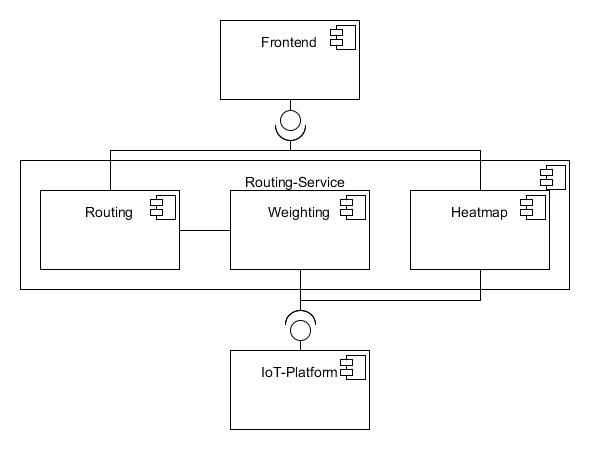
\includegraphics[width=\textwidth]{./ressourcen/routing/routingKomponenten.png}
	\caption{Grobe Architektur des RoutingService}
	\label{fig:routing_Komponenten}
\end{figure}

\Fig{routing_Komponenten} zeigt die zentralen Komponenten, die für den Routing Service benötigt werden, beziehungsweise die genutzt werden, um die im Routing Service benötigten Informationen und die daraus entstehenden Routen von der IoT-Plattform abzufragen oder auch die berechnete Route an das Frontend weiter zu geben. \\
Grundsätzlich besteht der Routing-Service selbst aus einer Routing-, einer Weighting- und einer Heatmap-Komponente. Die Routing-Komponente ist für die Errechnung der tatsächlichen Routen verantwortlich und die Weighting-Komponente sorgt für eine Gewichtung der einzelnen Kanten einer Route, sodass in der Gewichtung der Kanten auch Umweltgegebenheiten einfließen können. Eine klare Trennung der Routing- und Weighting-Komponente ist nicht möglich, da für ein umfassendes und präzises Routing immer eine detaillierte Kantengewichtung stattfinden muss.\\
Neben den beiden Hauptkomponenten gibt es die bereits erwähnten Schnittstellen zum Frontend sowie zur IoT-Plattform. Diese werden benötigt, um beispielsweise aktuell gemessene Umweltdaten in die Weighting-Komponente einfließen zu lassen. Weiterhin muss die Schnittstelle zum Frontend dafür sorgen, dass für ein Routing essentielle Informationen an den Routing-Service gelangen, wie beispielsweise der Start- und der Endpunkt der Route.\\
Anschließend an den Gesamtüberblick des Routing-Services soll in den folgenden Unterabschnitten der Aufbau der einzelnen Komponenten und Schnittstellen näher beleuchtet werden.


\subsection{Komponenten}
Die wohl zentralste Komponente des Routing-Services ist die Routing Komponente. Diese besteht im Wesentlichen aus der Erstellung einer Route, die dem Frontend per Schnittstelle zur Verfügung gestellt wird. Die Grundlage für die Berechnung einer Route ist das Einlesen von Kartenmaterial und die Generierung von Graphen durch das Framework Graphhopper (siehe dazu \Fref{sec:basics:routing:gh}).\\  
Um Routen berechnen zu können, müssen jedoch zuerst Informationen vom Navigationsnutzer vorgegeben werden. Dazu gehören zum Beispiel der Start- und Endpunkt der Route, das gewählt Fortbewegungsmittel sowie Angaben zu den Umweltparametern. Diese werden vom Frontend über einer HTTP-Schnittstelle entgegengenommen. 

\begin{figure}[htb]
	\centering
	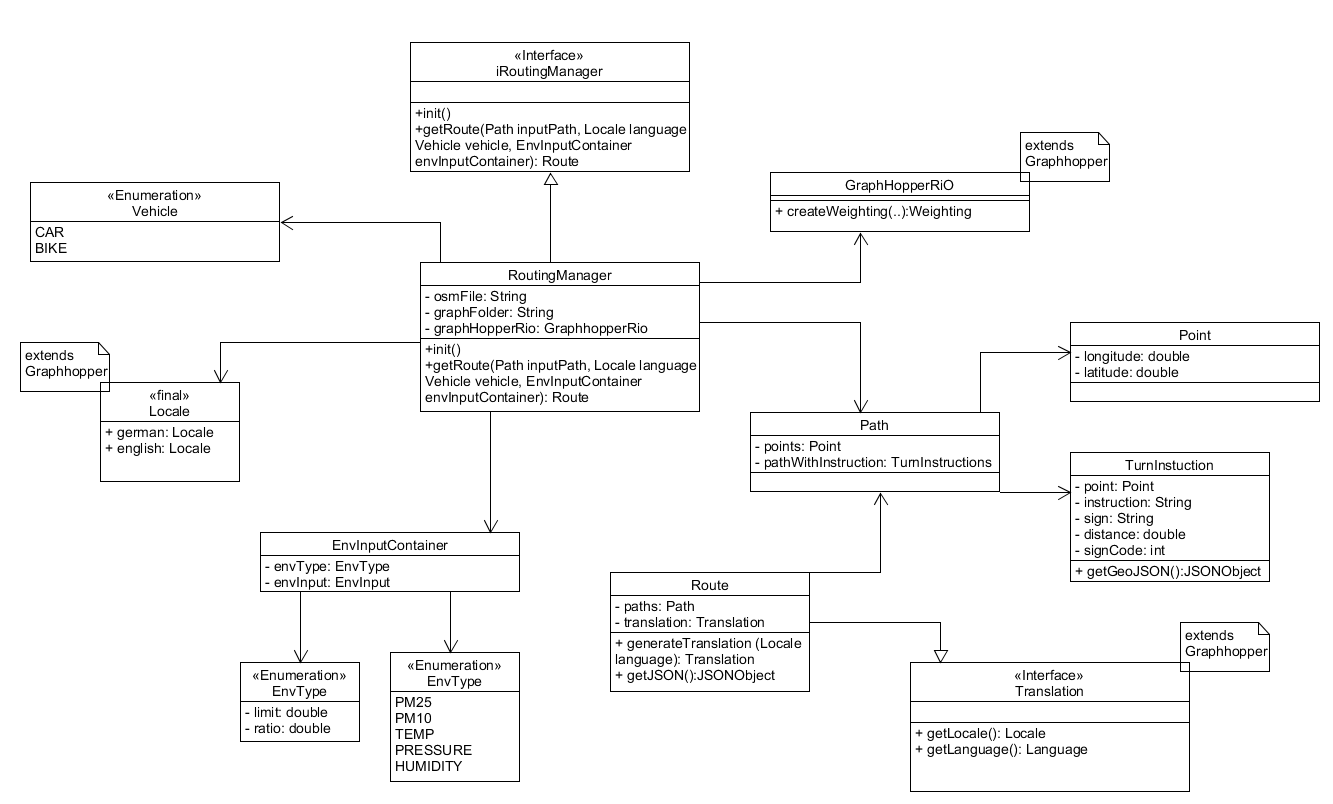
\includegraphics[width=\textwidth]{./ressourcen/routing/cdRouting.png}
	\caption{Grobe Architektur des RoutingService}
	\label{fig:routing_Klassendiagramm}
\end{figure}

\Fig{routing_Klassendiagramm} zeigt ein simples Diagramm, welches den grundsätzlichen Aufbau der Routing-Komponente beschreibt. Ausgangspunkt ist das Interface IRoutingManager, welches von der Klasse RoutingManager implementiert wird. Darin enthalten sind zwei Methoden, welche die Basis für die Berechnung von Routen liefern. Zum Einen gibt es die init-Methode. Diese wird zum Initialisieren des Singleton Routing Managers genutzt. Zum anderen gibt es die getRoute-Methode. Diese nimmt die benötigten Informationen von der Navigationsapplikation entgegen, lässt diese Informationen in eine Routenberechnung einfließen und gibt anschließend eine Route zurück. Um die getRoute-Methode aufzurufen müssen vom Frontend folgende Parameter an den Routing Service übergeben werden: ein inputPath, der die Navigationspunkte (zum Beispiel Start- und Endpunkt) enthält, die Sprache, auf der die Navigationsanweisungen später zurückgegeben werden, das Vehicle, sodass für dieses Fahrzeug spezifizierte Routen berechnet werden und die Umweltparameter, die in der Routenberechnung berücksichtigt werden sollen. Die daraufhin zurückgegebene Route besteht aus mindestens zwei Paths und einer Translation, wobei die Translation eine Methode ist, die von Graphhopper bereits zur Verfügung gestellt wird, um die Sprache für die Navigationsanweisung korrekt zurück zu geben. Ein Path hingegen besteht aus mindestens zwei Punkten: dem Längengrad und dem Breitengrad, die in der Klasse Point als double gespeichert werden sowie der TurnInstruction zu dem jeweiligen Path, welche Informationen speichert, wie die konkrete Navigationsanweisung (zum Beispiel "Turn Right"), die Distanz zur nächsten Anweisung und die geschätzte Zeit. All diese Informationen werden der Navigationsapplikation als ein GeoJSON-Format zurückgegeben. Dabei handelt es sich um ein spezielles JSON-Format, welches geometrische Informationen speichern kann.

Neben der Routing Komponenten ist der zweite zentrale Baustein des Routing-Services die Weighting-Komponente. Die stellt die Grundlage dazu dar, den Graphen mit überarbeiteten Gewichten zu versehen. Das Ziel dessen ist es, nicht nur die Distanz zweier Knoten zueinander als Gewicht in die Routenberechnung einfließen zu lassen, sondern das Gewicht durch Umweltdaten so zu verändern, dass zum Beispiel nicht die kürzeste Route berechnet wird, sondern eine Route, die sowohl die Feinstaubbelastung als auch die Distanz berücksichtigt. Dementsprechend muss die Möglichkeit geschaffen werden, das Gewicht einzelner Kanten zu beeinflussen, um die Umweltparameter einfließen zu lassen.
Die Basis für Berechnung der Gewichte sind die Werte der stationären Sensoren, die in Oldenburg ausgebracht werden sowie virtuelle Sensoren, die auf Basis Datenanalyse plausible Werte simulieren soll. Die Sensorwerte werden über eine Schnittstelle zur IoT-Plattform abgerufen.


\begin{figure}[htb]
	\centering
	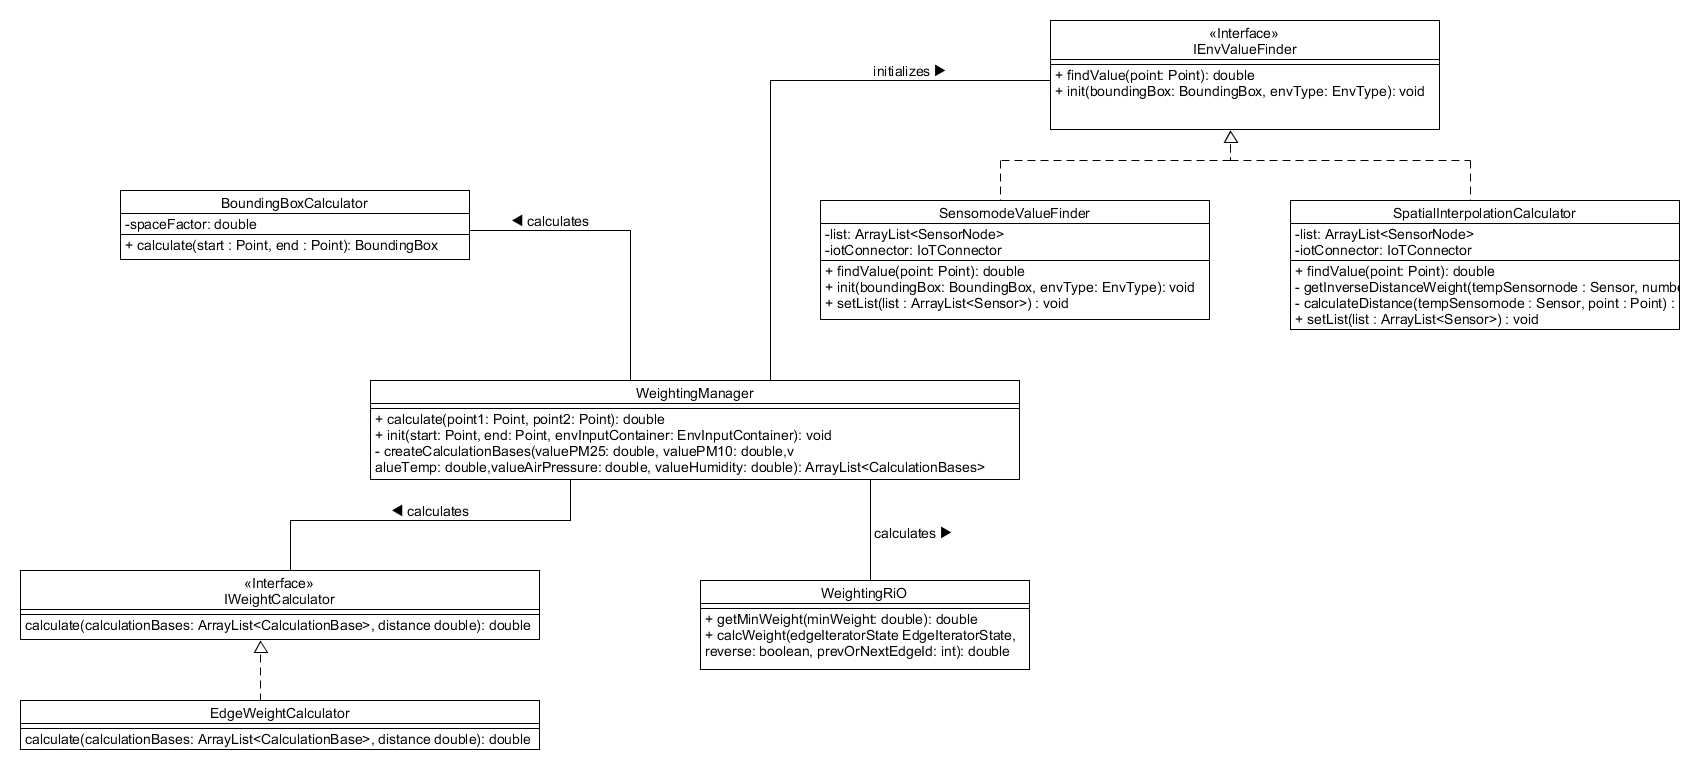
\includegraphics[width=\textwidth]{./ressourcen/routing/cdWeighting.png}
	\caption{Klassendiagramm Weighting-Komponente}
	\label{fig:weighting_Klassendiagramm}
\end{figure}


\Fig{weighting_Klassendiagramm} zeigt ein Diagramm der Weighting-Komponente mit den entsprechenden Klassen. Die zentrale Klasse, die den Weighting-Prozess steuert ist der WeightingManager. Dieser greift auf diverse andere Klassen zu und gibt letztendlich das Gewicht für jede Kante als double-Wert zurück. Dabei wird auf Basis der Eingabeparameter vom Frontend eine BoundingBox erzeugt, welche den abzufragenden Raum eingrenzt, in dem sich sinnvolle Sensorknoten befinden. Dieser Prozess wird in diesem Klassendiagramm durch die Klasse BoundingBoxCalculator repräsentiert. Um eine zu kleine BoundingBox zu verhindern, wird in dieser Klasse zusätzlich ein SpaceFactor gespeichert, der die BoundingBox um einen bestimmten Wert so verändert, dass diese selbst bei gleichen Längen- oder Breitengraden eine nützliche BoundingBox erzeugt (bei gleichen Längen- oder Breitengraden könnten sonst keine BoundingBox berechnet werden). 
Nachdem die BoundingBox kalkuliert wurde, wird das Interface IEnvValueFinder initialisiert, welches von der Klasse SensornodeValueFinder implementiert wird. In dieser wird eine Liste mit Sensorknoten angelegt, in welche die Sensorknoten eingetragen werden, welche sich innerhalb der zuvor berechneten BoundingBox befinden. Zum Initialisieren wird die init-Methode aufgerufen, in welche die BoundingBox sowie der EnvType eingegeben werden. Auf Basis dessen kann die findValue-Methode aufgerufen werden, in welche der Mittelpunkt einer Kante als Parameter eingegeben wird und die einen double-Wert zurückgibt, der den Umweltwert des am nächsten gelegenen Sensorknotens zu dem jeweiligen Eingabepunkt zurückgibt. 
Sobald die jeweiligen Umweltwerte der am nächsten gelegenen Sensorknoten gefunden wurden, wird das Interface IWeightCalculator aufgerufen, welches von der Klasse EdgeWeightCalculator implementiert wird. Diese Klasse ist dafür zuständig die einzelnen Kanten mit einem Gewicht zu versehen, welches zum Einen die Distanz berücksichtigt, welche des Gewicht abbildet, das von Graphhopper pro Kante generiert wird. Zum anderen wird für jede Kante der zuvor erhaltene Umweltwert mit in die Berechnung einbezogen. Dabei muss berücksichtigt werden, dass dem Navigationsnutzer die Möglichkeit gegeben wird, zusätzlich zu dem berücksichtigten Umweltwert, ein Limit für diesen Wert angegeben kann, sowie eine Gewichtung in Bezug auf andere Parameter. Hier kann es sich sowohl um weitere Umweltparameter handeln, als auch um die Distanz.
Schlussendlich wird für jede Kante ein Gewicht berechnet, welches die vorher erzeugten Werte einbezieht und so eine Gewichtung erzeugt, welche neben der Distanz auch Umweltparameter betrachten kann.

Neben der Routing- und der Weighting-Komponente verfügt der Routing-Service noch über einen dritten Baustein: der Heatmap-Komponente. Die Heatmap-Komponente hat im wesentlichen die Aufgabe, dem UIS-Frontend sowie der Navigationsapplikation einen Endpunkt bereitzustellen, über den diese eine Heatmap für einen bestimmten Bereich erhalten können. Eine Heatmap besteht dabei aus einem Raster an Werten, die aus den Messwerten der umliegenden Sensorknoten berechnet werden. 

\begin{figure}[htb]
	\centering
	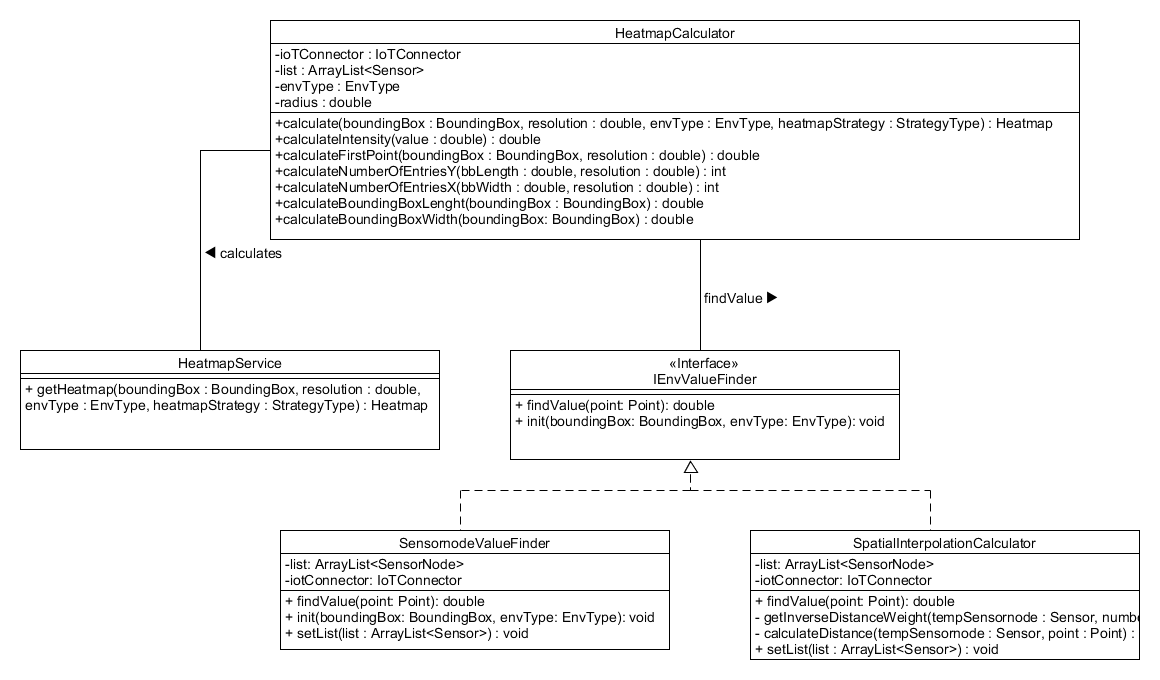
\includegraphics[width=\textwidth]{./ressourcen/routing/cdHeatmap.png}
	\caption{Klassendiagramm Heatmap-Komponente}
	\label{fig:heatmap_Klassendiagramm}
\end{figure}

In \Fig{heatmap_Klassendiagramm} sieht man ein Klassendiagramm, das die grundlegenden Klassen mit zugehörigen Methoden und Attribute der Heatmap-Komponente darstellt. Der Heatmap-Service verwaltet hierbei die Anfragen der Schnittstelle und leitet sie weiter an den HeatmapCalculator. Dieser fordert die notwendigen Sensorknotendaten bei der IoT-Plattform an und berechnet mit auf Basis der entsprechenden Werten der Sensorknoten die Heatmap. Bei der Berechnung wird zuerst die Anzahl der Einträge der Heatmap und der Aufbau (X und Y Einträge) berechnet. Danach werden iterativ die einzelnen Einträge der Heatmap berechnet. Hierfür wird aus der Liste aller Sensorknoten in dem gewünschten Bereich die Sensorkoten ausgewählt, die für den aktuellen Eintrag relevant sind. Für die Berechnung gibt es zwei verschiedene Strategien. Diese sind SensornodeValueFinder und SpatialInterpolationCalculator und implementieren das Interface IEnvValueFinder. Diese Unterscheiden sich in der Art der Zuordnung eines Feinstaubwertes zu einer Geoposition. 


Der SensornodeValueFinder berechnet die Distanz zwischen den einzelnen Sensorknoten und den Positionen in der Heatmap. Anschließend wird derjenige Sensorknoten ausgewählt, der die geringste Entfernung zur Position der Heatmap, der berechnet werden soll, hat. Der Position wird dann der Wert des ausgewählten Sensorknotens zugeordnet. Dieser Vorgang wird dann solang wiederholt, bis die Heatmap vollständig berechnet wurde.


Der SpatialInterpolationCalculator berechnet ebenso die Distanz zwischen den einzelnen Sensorknoten und den Positionen in der Heatmap. Anschließend wird eine Gewichtung für die einzelnen Sensorknoten aus der Distanz berechnet. Die Feinstaubwerte der Sensorknoten fließen dann zusammen mit der jeweiligen Gewichtung in die Berechnung des Heatmapeintrags mit ein.

\subsection{Schnittstellen}
Um zum Beispiel dem Frontend eine Route bereitzustellen, werden diverse Schnittstellen benötigt, die angeboten oder angesprochen werden. Im Folgenden ist daher eine nähere Beschreibung der Schnittstellen zu finden, die vom Routing-Service Richtung Frontend angeboten werden. Schnittstellen, die von der Weighting-Komponente konsumiert werden müssen, sind in den entsprechenden Architekturbeschreibungen definiert.

In der \Fig{ArchitekturRoutingSchnitstellen} sind die beiden Schnittstellen dargestellt, die von der Routing-Komponente angeboten werden müssen. 

\begin{figure}[htb]
	\centering
	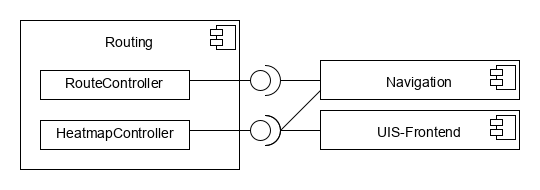
\includegraphics[width=\textwidth]{./ressourcen/routing/architekturRoutingSchnitstellen.png}
	\caption{Angebotene Schnittstellen der Routing-Komponente}
	\label{fig:ArchitekturRoutingSchnitstellen}
\end{figure}

Der \textit{RouteController} stellt die Schnittstelle zur Berechnung einer Route bereit. Als Eingabeparameter muss ein Fortbewegungsmittel, die Sprache, die Umweltparameter und die Punkte, an denen entlang geroutet werden sollen, angegeben werden. Die Umweltparameter setzen sich dabei aus einem Tripel zusammen, wobei der erste Wert den Umweltparameter, der zweite Wert den Grenzwert und der dritte Wert die Berücksichtigung in der Berechnung der Route benennt. Bei den Punkten müssen mindestens Start- und Endpunkt angegeben werden, es können aber auch bis zu drei Zwischenziele angegeben werden. Der \textit{RouteController} gibt dann, sofern eine Route gefunden werden konnte, eine Route im JSON-Format zurück. Ansonsten gibt es eine leere Antwort. Es kann auch alternative Routen geben, die dann auch mit zurückgegeben werden.

Der \textit{HeatmapController} stellt eine Heatmap für PM25-Werte bereit, welche dann sowohl im Frontend der Navigation als auch im Frontend für das Umweltinformationssystems dargestellt werden kann. Als Eingabe wird hier eine Strategie und eine sogenannte Bounding Box benötigt. Das sind zwei durch Latitude und Longitude definierte Punkte, die ein Viereck aufspannen. Die Heatmap, bestehend aus eine Menge von Punkten mit einer bestimmten Intensität, wird dann für diesen Bereich berechnet. Die Intensität pro Punkte, die sich im Wertebereich von null bis eins bewegt, gibt dann an, wie hoch der PM25-Wert in Relation zu den anderen Punkten der Heatmap sind. Die Berechnung dieser Punkte können unterschiedliche Strategien zugrunde liegen, welche durch den zweiten Eingabeparameter festgelegt werden. Ebenso wie die Route des \textit{RouteControllers} wird auch die Heatmap im JSON-Format zurück gegeben.

\subsection{Ablauf einer Routing-Anfrage}
In diesem Abschnitt soll der gesamte Ablauf zur Erstellung einer Route dargestellt werden. Dieser ist in \Fig{Routinganfrage_Sequenzdiagramm} dargestellt. Es handelt sich dabei nur um synchrone Aufrufe, sodass die eingehende Anfrage durch verschiedene Klassen und Methoden geleitet wird, bevor die erstellte Route an die Navigationsapplikation weitergegeben werden kann.

\begin{figure}[htb]
	\centering
	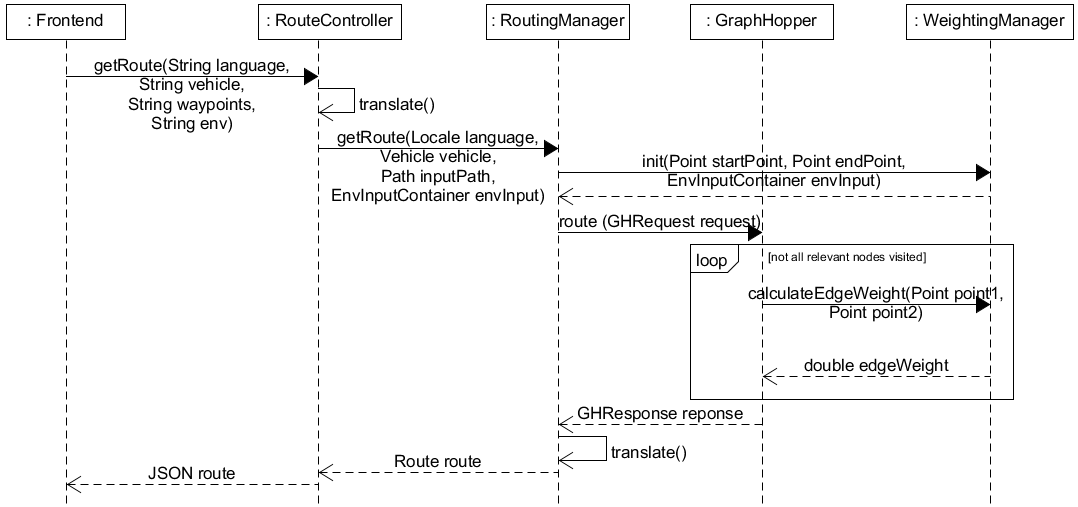
\includegraphics[width=\textwidth]{./ressourcen/routing/sdAbfrage.png}
	\caption{Sequenzdiagramm Routinganfrage}
	\label{fig:Routinganfrage_Sequenzdiagramm}
\end{figure}

Grob betrachtet spielen sechs Klassen eine Rolle zur Erstellung einer Route, wobei diese üblicherweise mehrere Klassen ansprechen, auf welche in diesem Sequenzdiagramm auf Grund der Übersichtlichkeit nicht näher eingegangen wird. Zum Aufbau der Klassen siehe \Fig{routing_Klassendiagramm} und \Fig{weighting_Klassendiagramm}. Weiterhin wird im Sequenzdiagramm das Frontend als Klasse dargestellt, obwohl dies keine eigene Klasse im Routing Service darstellt. Gemeint ist die Navigationsapplikation, welche die Routing-Anfrage an den Routing Service stellt. \\
Zuerst stellt das Frontend eine Routing-Anfrage an den RouteController, in welchem die getRoute-Methode aufgerufen wird. Dafür müssen folgende Informationen in der Anfrage gepflegt sein: die Navigationspunkte, die Sprache, das Vehicle und die zu berücksichtigen Umweltparamter. Diese Informationen werden als String an den RouteController übergeben. Daraufhin werden die Strings der Anfrage in andere Typen übersetzt, die von dem Routing Service genutzt werden können. Dies geschieht in der Translate-Klassen. Daran anschließend ruft der RouteController die getRoute-Methode der Klasse RoutingManager auf, in welchem die übersetzten Variablen eingegeben werden. Dieser ruft die init-Methode des WeightingManagers auf, um ebendiesen zu initialisieren. Nachdem der WeightingManager initialisiert wurde, wird die route-Methode von Graphhopper aufgerufen. In dieser werden die Kantengewichte des Graphen berechnet, um auf Basis dieser Kantengewichte die möglichen Routen zu berechnen. Diese Funktion wird für jede Kante einzeln aufgerufen, sodass jede Kante anschließend mit einem Gewicht versehen ist.\\
Die daraus entstehende Antwort wird vom RoutingManager so übersetzt, dass die Antwort als Route an den RouteController übergeben werden kann, welche aus der Antwort eine JSON-Datei erstellt, die schlussendlich an die Navigationsapplikation zurückgegeben wird.
